  % ============================================================
  %  CHAPTER 3 — METHODOLOGY
  % ============================================================

  This chapter presents the methodological framework underlying the design and                                                                            
  implementation of \textbf{UrbanPulse}, a streaming-first urban intelligence
  platform for Ho Chi Minh City. The chapter is organized as follows.                                                                                     
  Section~\ref{sec:requirements} establishes the functional and non-functional
  requirements through use case analysis. Section~\ref{sec:ingestion} describes                                                                           
  the data acquisition and ingestion strategy. Section~\ref{sec:medallion}
  details the multi-stage \textit{Medallion Architecture} for stream processing                                                                           
  and data transformation. Section~\ref{sec:anomaly} formalizes the                                                                                       
  \textbf{dual-signal anomaly detection framework}. Section~\ref{sec:rag}                                                                                 
  presents the \textit{Retrieval-Augmented Generation} (RAG) pipeline for                                                                                 
  knowledge-enriched inference. Finally, Section~\ref{sec:evaluation} defines                                                                             
  the evaluation framework and key performance indicators used in Chapter~4.                                                                              
                                                                                                                                                          
  % ============================================================
  \section{Requirement Analysis}                                                                                                                          
  \label{sec:requirements}
  % ============================================================                                                                                          
   
  The requirements of UrbanPulse are derived from the operational needs of                                                                                
  municipal traffic management in a large Southeast Asian metropolitan area.
  Ho Chi Minh City presents a particularly demanding environment: a
  metropolitan population of approximately 8~million, with personal vehicles
  serving up to 85\% of daily travel needs and peak-hour congestion
  patterns that shift substantially across zones, time of day, and
  meteorological conditions \cite{hcmc_transport_report}.                                                                  
  Existing monitoring approaches rely on periodic batch reporting, introducing                                                                            
  temporal gaps of up to several hours between event occurrence and situational                                                                           
  awareness \cite{batch_latency_survey}. UrbanPulse is designed to close this                                                                             
  gap through continuous ingestion, real-time feature computation, and                                                                                    
  LLM-assisted root cause analysis.                                                                                                                       
                                                                                                                                                          
  % ------------------------------------------------------------                                                                                          
  \subsection{Functional Requirements}
  \label{subsec:functional_req}                                                                                                                           
  % ------------------------------------------------------------
                                                                                                                                                          
  The following functional requirements were identified through analysis of                                                                               
  urban traffic management workflows:
                                                                                                                                                          
  \begin{enumerate}
      \item \textbf{FR-1 Continuous Data Ingestion:} The system shall
      continuously acquire route-level traffic observations from a commercial                                                                             
      mapping API and publish them to a durable, replayable message log with                                                                              
      sub-minute freshness.                                                                                                                               
                                                                                                                                                          
      \item \textbf{FR-2 Real-Time Feature Computation:} For each ingested                                                                                
      observation, the system shall compute and persist route-level statistical
      features (mean duration, heavy vehicle ratio, standard deviation) within                                                                            
      20 seconds of message arrival.                                                                                                                      
                                                                                                                                                          
      \item \textbf{FR-3 Anomaly Detection:} The system shall classify each                                                                               
      route observation as anomalous or normal using at least two independent                                                                             
      detection methods, and expose the results through a queryable REST API.                                                                             
                                                                                                                                                          
      \item \textbf{FR-4 Historical Analytics:} The system shall maintain a                                                                               
      versioned, queryable history of all traffic observations at Bronze,                                                                                 
      Silver, and Gold granularity, supporting point-in-time queries for                                                                                  
      reproducible analysis.
                                                                                                                                                          
      \item \textbf{FR-5 Explainability:} The system shall provide
      human-readable natural-language explanations of detected anomalies,                                                                                 
      grounded in historical context and meteorological conditions.                                                                               
                                                                                                                                                          
      \item \textbf{FR-6 Automated Alerting:} The system shall deliver                                                                                    
      push notifications for high-confidence anomaly events with configurable                                                                             
      per-route cooldown periods to suppress duplicate alerts.                                                                                            
  \end{enumerate}                                                                                                                                         
                                                                                                                                                          
  % ------------------------------------------------------------                                                                                          
  \subsection{Non-Functional Requirements}
  \label{subsec:nonfunctional_req}
  % ------------------------------------------------------------                                                                                          
   
  \begin{enumerate}                                                                                                                                       
      \item \textbf{NFR-1 Latency:} End-to-end ingestion lag (API response
      to persisted feature) shall not exceed 20 seconds at the 95th percentile                                                                            
      under normal operating load.                                                                                                                        
                                                                                                                                                          
      \item \textbf{NFR-2 Reproducibility:} Any anomaly classification                                                                                    
      produced by the system shall be reproducible by querying the exact                                                                                  
      Lakehouse snapshot and MLflow model version active at the time of                                                                                   
      inference.                                                                                                                                          
                                                                                                                                                          
      \item \textbf{NFR-3 Fault Tolerance:} The ingestion and feature                                                                                     
      computation pipelines shall tolerate transient service failures without
      data loss, through Kafka offset management and Postgres-based                                                                                       
      accumulator recovery.                                                                                                                               
                                                                                                                                                          
      \item \textbf{NFR-4 Scalability:} The architecture shall be horizontally                                                                            
      scalable at the ingestion and serving layers without modification to                                                                                
      the core processing logic.                                                                                                                          
   
      \item \textbf{NFR-5 Observability:} All system components shall emit                                                                                
      structured logs, metrics, and traces consumable by a centralised
      monitoring stack.                                                                                                                                   
  \end{enumerate} 
                                                                                                                                                          
  % ------------------------------------------------------------
  \subsection{Use Case Description}
  \label{subsec:use_case_desc}
  % ------------------------------------------------------------

  Table~\ref{tab:use_cases} summarises the primary actors and their                                                                                       
  interactions with the UrbanPulse platform.
                                                                                                                                                          
  \begin{table}[h]
  \centering                                                                                                                                              
  \caption{Primary use cases and actors in UrbanPulse}
  \label{tab:use_cases}
  \begin{tabular}{lll}                                                                                                                                    
  \hline
  \textbf{Use Case} & \textbf{Actor} & \textbf{Trigger} \\                                                                                                
  \hline          
  Monitor live traffic map      & Traffic operator  & Continuous / 15-second refresh \\                                                                   
  Investigate anomaly           & Traffic analyst   & Alert notification received \\
  Request root cause analysis   & Traffic analyst   & Manual query via dashboard \\                                                                       
  Review historical trend       & Urban planner     & Ad-hoc query \\                                                                                     
  Receive anomaly alert         & Duty manager      & Automated Telegram notification \\                                                                  
  Retrain detection model       & ML engineer       & Scheduled (every 6 hours) \\                                                                        
  \hline                                                                                                                                                  
  \end{tabular}                                                                                                                                           
  \end{table}                                                                                                                                             
                                                                                                                                                          
  % ------------------------------------------------------------
  \subsection{Use Case Diagram}                                                                                                                           
  \label{subsec:use_case_diagram}
  % ------------------------------------------------------------

  Figure~\ref{fig:use_case} illustrates the relationships between system                                                                                  
  actors and use cases. The \textit{Traffic Operator} and \textit{Traffic
  Analyst} interact primarily with the Serving API layer, whilst the                                                                                      
  \textit{ML Engineer} interacts with the batch orchestration layer.                                                                                      
  The \textit{External APIs} actor represents the automated data sources                                                                                  
  (VietMap and Open-Meteo) that trigger the ingestion pipeline.                                                                                           
                                                                                                                                                          
  \begin{figure}[h]                                                                                                                                       
      \centering                                                                                                                                          
      \resizebox{0.95\textwidth}{!}{%
      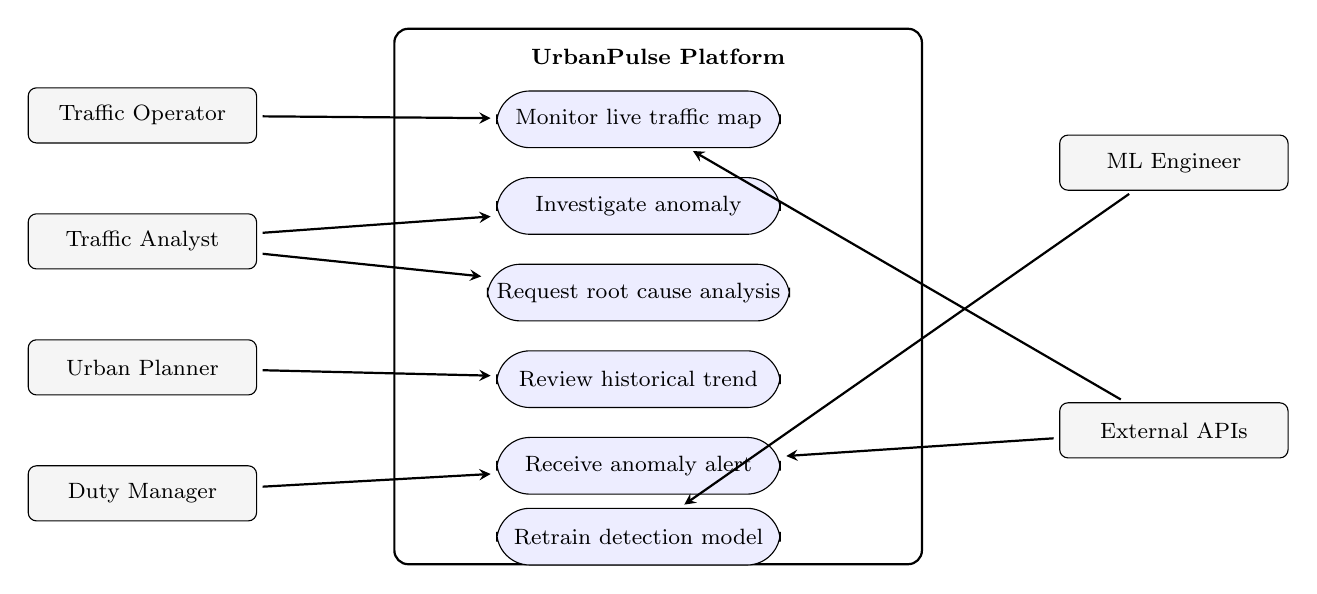
\begin{tikzpicture}[
        >=stealth,
        actor/.style={draw, rounded corners=3pt, fill=gray!8,
                      minimum width=2.9cm, minimum height=0.7cm,
                      align=center, font=\footnotesize},
        usecase/.style={draw, rounded corners=12pt, fill=blue!7,
                        minimum width=3.6cm, minimum height=0.72cm,
                        align=center, font=\footnotesize},
        arr/.style={->, thick, shorten >=2pt, shorten <=2pt}
      ]
        \draw[rounded corners=5pt, thick] (-3.1,-3.4) rectangle (3.6,3.4);
        \node[font=\bfseries\footnotesize] at (0.25,3.05) {UrbanPulse Platform};

        \node[actor] (operator) at (-6.3,2.3) {Traffic Operator};
        \node[actor] (analyst)  at (-6.3,0.7) {Traffic Analyst};
        \node[actor] (planner)  at (-6.3,-0.9) {Urban Planner};
        \node[actor] (manager)  at (-6.3,-2.5) {Duty Manager};
        \node[actor] (mleng)    at (6.8,1.7) {ML Engineer};
        \node[actor] (external) at (6.8,-1.7) {External APIs};

        \node[usecase] (monitor) at (0,2.25) {Monitor live traffic map};
        \node[usecase] (invest)  at (0,1.15) {Investigate anomaly};
        \node[usecase] (rca)     at (0,0.05) {Request root cause analysis};
        \node[usecase] (trend)   at (0,-1.05) {Review historical trend};
        \node[usecase] (alert)   at (0,-2.15) {Receive anomaly alert};
        \node[usecase] (retrain) at (0,-3.05) {Retrain detection model};

        \draw[arr] (operator) -- (monitor);
        \draw[arr] (analyst) -- (invest);
        \draw[arr] (analyst) -- (rca);
        \draw[arr] (planner) -- (trend);
        \draw[arr] (manager) -- (alert);
        \draw[arr] (mleng) -- (retrain);
        \draw[arr] (external) -- (monitor);
        \draw[arr] (external) -- (alert);
      \end{tikzpicture}%
      }
      \caption{Use case diagram for the UrbanPulse platform.}
      \label{fig:use_case}                                                                                                                                
  \end{figure}    
                                                                                                                                                          
  % ------------------------------------------------------------
  \subsection{System Overview}
  \label{subsec:system_overview}                                                                                                                          
  % ------------------------------------------------------------
                                                                                                                                                          
  Figure~\ref{fig:architecture} presents the high-level architecture of
  UrbanPulse. The platform is structured into four horizontal layers:
  the \textit{Ingestion Layer}, the \textit{Processing Layer}, the                                                                                        
  \textit{Serving Layer}, and the \textit{Inference Layer}. Data flows                                                                                    
  vertically from external APIs through the \textbf{Redpanda} message broker                                                                              
  — a \textit{Kafka}-compatible distributed streaming platform                                                                                            
  \cite{redpanda_whitepaper} — into two parallel consumer paths: a                                                                                        
  \textit{durable archival path} that materialises data into a versioned                                                                                  
  \textbf{Data Lakehouse}, and a \textit{real-time feature path} that writes                                                                              
  statistical summaries to \textbf{PostgreSQL} for low-latency serving.                                                                                   
  The Serving Layer exposes a REST and Server-Sent Events (SSE) API surface.                                                                              
  The Inference Layer augments API responses with LLM-generated explanations                                                                              
  produced by a locally hosted \textbf{Qwen2.5:3b} model via                                                                                              
  \textbf{Ollama} \cite{qwen25_report}.                                                                                                                   
                  
  \begin{figure}[htbp]
  \centering
  \resizebox{\textwidth}{!}{%
  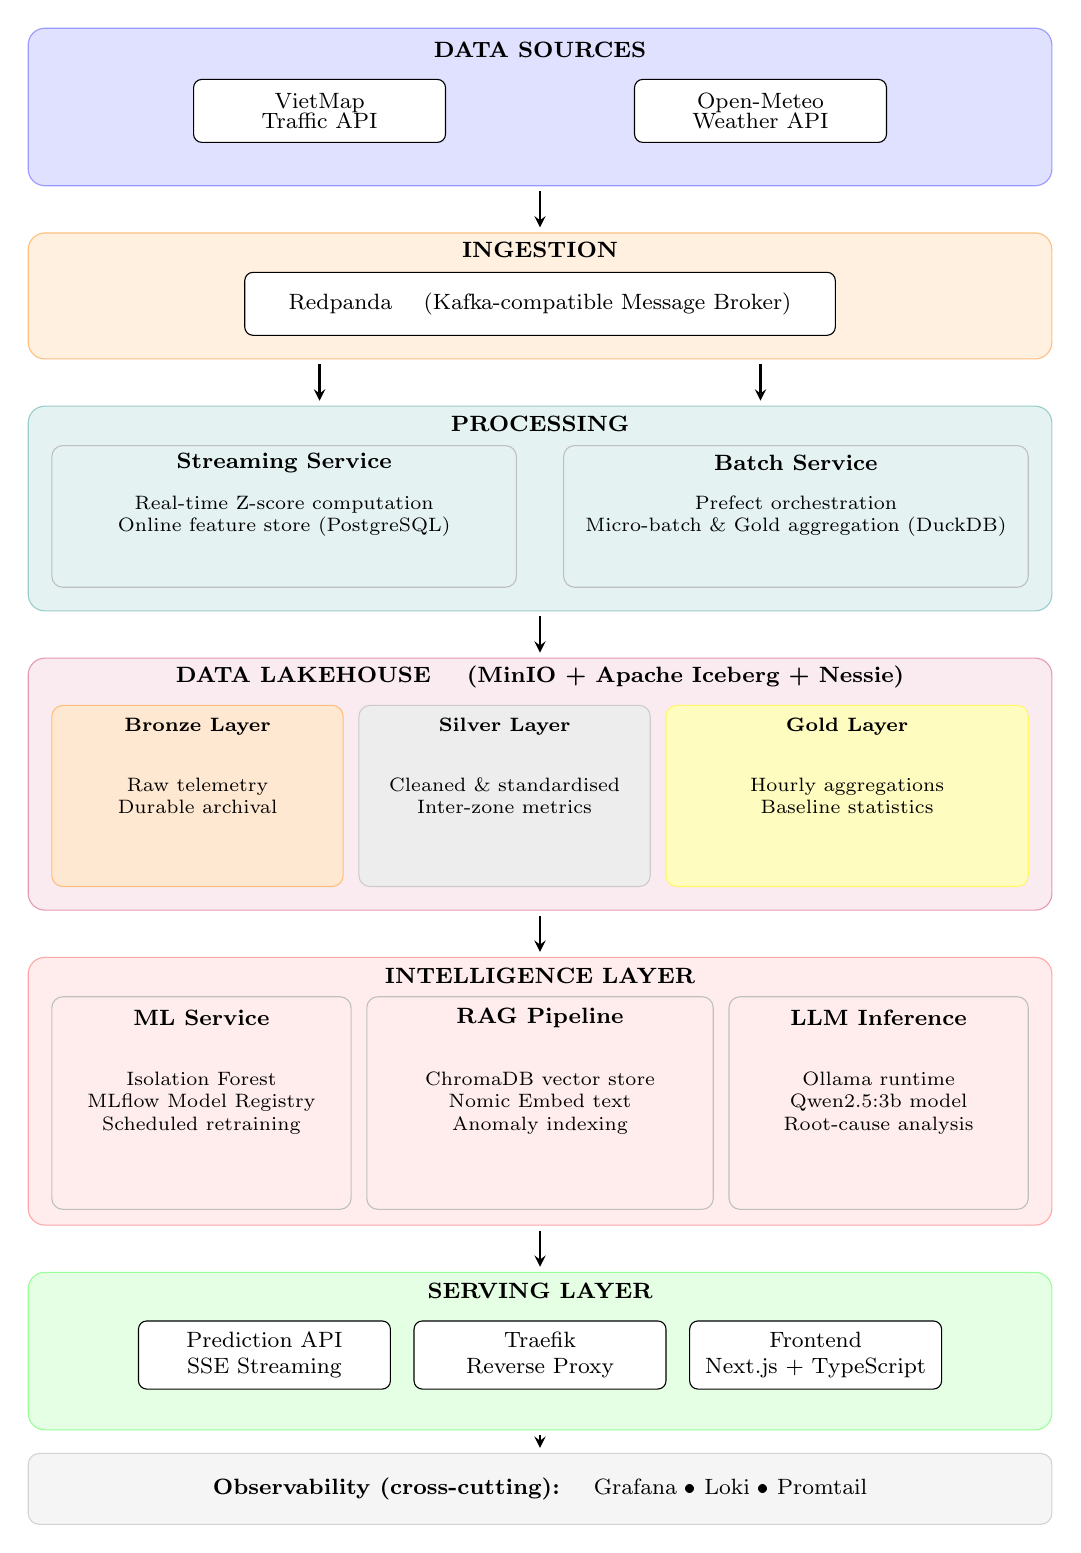
\begin{tikzpicture}[
    >=stealth, font=\small,
    cbox/.style={draw, rounded corners=3pt, fill=white,
                 minimum width=3.2cm, minimum height=0.8cm,
                 align=center, font=\footnotesize, inner sep=4pt},
    arr/.style={->, thick, shorten >=2pt, shorten <=2pt},
    llabel/.style={font=\bfseries\footnotesize}
  ]

  %% ── Layer 1: Data Sources ──
  \fill[blue!12, rounded corners=6pt] (-6.5,-1.0) rectangle (6.5,1.0);
  \draw[blue!40,  rounded corners=6pt] (-6.5,-1.0) rectangle (6.5,1.0);
  \node[llabel] at (0, 0.72) {DATA SOURCES};
  \node[cbox] at (-2.8,-0.05) {VietMap\\[-2pt]Traffic API};
  \node[cbox] at ( 2.8,-0.05) {Open-Meteo\\[-2pt]Weather API};

  \draw[arr] (0,-1.0) -- (0,-1.6);

  %% ── Layer 2: Ingestion ──
  \fill[orange!12, rounded corners=6pt] (-6.5,-3.2) rectangle (6.5,-1.6);
  \draw[orange!50, rounded corners=6pt] (-6.5,-3.2) rectangle (6.5,-1.6);
  \node[llabel] at (0,-1.82) {INGESTION};
  \node[draw, rounded corners=3pt, fill=white, minimum width=7.5cm,
        minimum height=0.8cm, align=center, font=\footnotesize, inner sep=4pt]
    at (0,-2.5) {Redpanda \quad (Kafka-compatible Message Broker)};

  \draw[arr] (-2.8,-3.2) -- (-2.8,-3.8);
  \draw[arr] ( 2.8,-3.2) -- ( 2.8,-3.8);

  %% ── Layer 3: Processing ──
  \fill[teal!10, rounded corners=6pt] (-6.5,-6.4) rectangle (6.5,-3.8);
  \draw[teal!40,  rounded corners=6pt] (-6.5,-6.4) rectangle (6.5,-3.8);
  \node[llabel] at (0,-4.02) {PROCESSING};

  \draw[gray!50, rounded corners=4pt] (-6.2,-6.1) rectangle (-0.3,-4.3);
  \node[font=\footnotesize\bfseries] at (-3.25,-4.52) {Streaming Service};
  \node[font=\scriptsize, align=center] at (-3.25,-5.2)
      {Real-time Z-score computation\\Online feature store (PostgreSQL)};

  \draw[gray!50, rounded corners=4pt] (0.3,-6.1) rectangle (6.2,-4.3);
  \node[font=\footnotesize\bfseries] at (3.25,-4.52) {Batch Service};
  \node[font=\scriptsize, align=center] at (3.25,-5.2)
      {Prefect orchestration\\Micro-batch \& Gold aggregation (DuckDB)};

  \draw[arr] (0,-6.4) -- (0,-7.0);

  %% ── Layer 4: Data Lakehouse ──
  \fill[purple!8,  rounded corners=6pt] (-6.5,-10.2) rectangle (6.5,-7.0);
  \draw[purple!40, rounded corners=6pt] (-6.5,-10.2) rectangle (6.5,-7.0);
  \node[llabel] at (0,-7.24) {DATA LAKEHOUSE \quad (MinIO + Apache Iceberg + Nessie)};

  \fill[orange!18, rounded corners=4pt] (-6.2,-9.9) rectangle (-2.5,-7.6);
  \draw[orange!50, rounded corners=4pt] (-6.2,-9.9) rectangle (-2.5,-7.6);
  \node[font=\scriptsize\bfseries] at (-4.35,-7.87) {Bronze Layer};
  \node[font=\scriptsize, align=center] at (-4.35,-8.75)
      {Raw telemetry\\Durable archival};

  \fill[gray!14, rounded corners=4pt] (-2.3,-9.9) rectangle (1.4,-7.6);
  \draw[gray!40,  rounded corners=4pt] (-2.3,-9.9) rectangle (1.4,-7.6);
  \node[font=\scriptsize\bfseries] at (-0.45,-7.87) {Silver Layer};
  \node[font=\scriptsize, align=center] at (-0.45,-8.75)
      {Cleaned \& standardised\\Inter-zone metrics};

  \fill[yellow!25, rounded corners=4pt] (1.6,-9.9) rectangle (6.2,-7.6);
  \draw[yellow!60, rounded corners=4pt] (1.6,-9.9) rectangle (6.2,-7.6);
  \node[font=\scriptsize\bfseries] at (3.9,-7.87) {Gold Layer};
  \node[font=\scriptsize, align=center] at (3.9,-8.75)
      {Hourly aggregations\\Baseline statistics};

  \draw[arr] (0,-10.2) -- (0,-10.8);

  %% ── Layer 5: Intelligence ──
  \fill[red!7,  rounded corners=6pt] (-6.5,-14.2) rectangle (6.5,-10.8);
  \draw[red!35, rounded corners=6pt] (-6.5,-14.2) rectangle (6.5,-10.8);
  \node[llabel] at (0,-11.04) {INTELLIGENCE LAYER};

  \draw[gray!50, rounded corners=4pt] (-6.2,-14.0) rectangle (-2.4,-11.3);
  \node[font=\footnotesize\bfseries] at (-4.3,-11.57) {ML Service};
  \node[font=\scriptsize, align=center] at (-4.3,-12.65)
      {Isolation Forest\\MLflow Model Registry\\Scheduled retraining};

  \draw[gray!50, rounded corners=4pt] (-2.2,-14.0) rectangle (2.2,-11.3);
  \node[font=\footnotesize\bfseries] at (0,-11.57) {RAG Pipeline};
  \node[font=\scriptsize, align=center] at (0,-12.65)
      {ChromaDB vector store\\Nomic Embed text\\Anomaly indexing};

  \draw[gray!50, rounded corners=4pt] (2.4,-14.0) rectangle (6.2,-11.3);
  \node[font=\footnotesize\bfseries] at (4.3,-11.57) {LLM Inference};
  \node[font=\scriptsize, align=center] at (4.3,-12.65)
      {Ollama runtime\\Qwen2.5:3b model\\Root-cause analysis};

  \draw[arr] (0,-14.2) -- (0,-14.8);

  %% ── Layer 6: Serving ──
  \fill[green!10, rounded corners=6pt] (-6.5,-16.8) rectangle (6.5,-14.8);
  \draw[green!40, rounded corners=6pt] (-6.5,-16.8) rectangle (6.5,-14.8);
  \node[llabel] at (0,-15.04) {SERVING LAYER};
  \node[cbox] at (-3.5,-15.85) {Prediction API\\SSE Streaming};
  \node[cbox] at (0,  -15.85) {Traefik\\Reverse Proxy};
  \node[cbox] at ( 3.5,-15.85) {Frontend\\Next.js + TypeScript};

  %% ── Observability banner ──
  \draw[arr, dashed] (0,-16.8) -- (0,-17.1);
  \fill[gray!8,  rounded corners=4pt] (-6.5,-18.0) rectangle (6.5,-17.1);
  \draw[gray!35, rounded corners=4pt] (-6.5,-18.0) rectangle (6.5,-17.1);
  \node[font=\footnotesize, align=center] at (0,-17.55)
      {\textbf{Observability (cross-cutting):} \quad
       Grafana \textbullet{} Loki \textbullet{} Promtail};

  \end{tikzpicture}%
  }
  \caption{High-level system architecture of UrbanPulse.}
  \label{fig:architecture}
  \end{figure}
                                                                                                                                                          
  % ============================================================
  \clearpage
  \section{Data Acquisition and Ingestion Strategy}
  \label{sec:ingestion}                                                                                                                                   
  % ============================================================
                                                                                                                                                          
  Reliable, low-latency data acquisition is the foundation upon which all                                                                                 
  downstream processing depends. This section describes the two data sources
  integrated by UrbanPulse and the mechanism by which raw API responses are                                                                               
  converted into a replayable event stream.                                                                                                               
                                                                                                                                                          
  % ------------------------------------------------------------                                                                                          
  \subsection{Traffic Telemetry — VietMap Directions API}
  \label{subsec:vietmap}                                                                                                                                  
  % ------------------------------------------------------------
                                                                                                                                                          
  Route-level traffic observations are acquired by periodically polling the
  \textbf{VietMap Directions API} \cite{vietmap_api}, a commercial Vietnamese                                                                             
  mapping provider with national road network coverage. The ingestion service                                                                             
  iterates over the set of inter-zone routes defined in a canonical                                                                                      
  \texttt{routes.json} configuration file. Routes are generated from a                                                                                    
  \texttt{zones.json} specification that partitions Ho Chi Minh City into six                                                                             
  functional zones: \textit{Urban Core}, \textit{Eastern Innovation},                                                                                     
  \textit{Northern Industrial}, \textit{Southern Port},                                                                                                   
  \textit{Western Peri-urban}, and \textit{Southern Coastal}. Each route is                                                                               
  expressed as a directed pair of origin and destination zone anchors.                                                                                    
  The route set is an operational subset of the full directed zone-pair                                                                                   
  space, selected to cover the major radial and cross-city corridors while                                                                                
  keeping the dashboard and alert surface interpretable for thesis-scale                                                                                  
  evaluation.                                                                                    
                                                                                                                                                          
  For each route, a single API call returns the following fields: travel                                                                                  
  duration $d_r$ (minutes), distance $\delta_r$ (metres), and a congestion                                                                                
  breakdown comprising four segment-level ratios. Let $S_r$ denote the set                                                                                
  of road segments on route $r$. The congestion features are:                                                                                             
                                                                                                                                                          
  \begin{equation}                                                                                                                                        
  \label{eq:heavy_ratio}                                                                                                                                  
  \text{heavy\_ratio}_r = \frac{|\{s \in S_r : \text{level}(s) = \text{heavy}\}|}{|S_r|}
  \end{equation}                                                                                                                                          
   
  with analogous definitions for $\text{moderate\_ratio}_r$,                                                                                              
  $\text{low\_ratio}_r$, and $\text{severe\_segments}_r$ (absolute count).
  A 10-second inter-request delay between consecutive API calls is enforced                                                                               
  to comply with rate-limit constraints. A complete crawl cycle across all                                                                                
  routes completes within the 5-minute polling interval.                                                                                               
                                                                                                                                                          
  It is important to clarify that VietMap operates as a \textbf{polling-based                                                                             
  source} rather than a push-based event stream. The ingestion service
  bridges this gap by publishing each validated observation immediately to                                                                                
  Redpanda via the Kafka producer protocol, effectively converting a                                                                                      
  batch API into a synthetic event stream. This pattern decouples the                                                                                     
  polling schedule from all downstream consumers: the pipeline behaves                                                                                    
  as a true streaming system regardless of source polling frequency                                                                                       
  \cite{kleppmann_ddia}.                                                                                                                                  
                                                                                                                                                          
  Each API response is published to two Kafka topics: the raw VietMap                                                   
  response bytes are forwarded as-is to \texttt{vietmap-raw}; a                                                         
  transformed representation with extracted route metrics and computed                                                  
  congestion ratios is published to \texttt{traffic-route-bronze}.                                                      
  Both messages carry the same \texttt{ingest\_ts} header --- the Unix                                                  
  epoch millisecond timestamp recorded immediately before the API call ---                                              
  which serves as the reference point for end-to-end latency measurement                                                
  in all downstream consumers.                                                                                                 
                                                                                                                                                          
  % ------------------------------------------------------------
  \subsection{Meteorological Context — Open-Meteo API}                                                                                                    
  \label{subsec:openmeteo}
  % ------------------------------------------------------------                                                                                          
   
  Hourly weather data is retrieved from the \textbf{Open-Meteo API}
  \cite{openmeteo_api}, a free, open-source meteorological service
  requiring no authentication. The \texttt{weather-ingestion} service
  polls Open-Meteo every 15 minutes ($\texttt{\_CYCLE\_INTERVAL\_S} = 900$)
  for all \textbf{six} zone-specific coordinates independently
  (Table~\ref{tab:zone_coords}), publishing one \texttt{WeatherObservation}
  per zone per cycle to Kafka. Retrieved variables include:
  temperature ($^\circ$C), precipitation ($\text{mm}$), rainfall
  ($\text{mm}$), wind speed ($\text{km/h}$), wind direction ($^\circ$),
  cloud cover ($\%$), and WMO weather code.

  \begin{table}[h]
  \centering
  \caption{Zone-specific Open-Meteo query coordinates.}
  \label{tab:zone_coords}
  \small
  \begin{tabular}{llcc}
  \hline
  \textbf{Zone ID} & \textbf{Name} & \textbf{Latitude} & \textbf{Longitude} \\
  \hline
  zone1 & Urban Core           & $10.7755^\circ$N & $106.6990^\circ$E \\
  zone2 & Eastern Innovation   & $10.8667^\circ$N & $106.7793^\circ$E \\
  zone3 & Northern Industrial  & $11.1031^\circ$N & $106.5496^\circ$E \\
  zone4 & Southern Port        & $10.7630^\circ$N & $106.7722^\circ$E \\
  zone5 & Western Peri-urban   & $10.6867^\circ$N & $106.5774^\circ$E \\
  zone6 & Southern Coastal     & $10.5842^\circ$N & $107.0368^\circ$E \\
  \hline
  \end{tabular}
  \end{table}

  Weather data is consumed in two operationally distinct modes:

  \begin{enumerate}
      \item \textbf{Batch indexing mode:} Zone-level observations flow
      from Kafka into the batch pipeline, which averages them into a
      single city-level record per hour and persists the result to the
      \texttt{gold.weather\_hourly} Iceberg table. The RAG indexer
      then reads the trailing 7 days from this table
      ($\approx 192$ documents) and upserts them into the
      \texttt{external\_\allowbreak context} ChromaDB collection
      (Section~\ref{sec:rag}). A direct Open-Meteo API fallback is
      used only when \texttt{gold.weather\_hourly} is not yet
      available (e.g.\ during initial bootstrap).

      \item \textbf{Live fetch mode:} On each \texttt{/chat} API request,
      the serving layer performs a direct asynchronous HTTP fetch of
      current conditions using a single city-centre coordinate
      ($10.7757^\circ$N, $106.7009^\circ$E), cached in-process for
      15 minutes, and injects the result into the LLM system prompt.
  \end{enumerate}                                                                                                                                         
                                                                                                                                                          
  Weather data is \textbf{not} used as an input to either anomaly detection                                                                               
  model. Its role is exclusively contextual enrichment for the LLM
  inference layer described in Section~\ref{sec:rag}.                                                                                                     
                                                                                                                                                          
  % ============================================================                                                                                          
  \section{Stream Processing and Medallion Architecture}                                                                                                  
  \label{sec:medallion}
  % ============================================================

  Once published to Redpanda, traffic observations are consumed by two                                                                                    
  independent consumer groups operating in parallel — one for durable
  archival, one for real-time feature computation. This fan-out architecture,                                                                             
  illustrated in Figure~\ref{fig:data_flow}, ensures that neither path                                                                                    
  can block or slow the other. The following subsections describe each                                                                                    
  processing stage in the \textbf{Medallion Architecture}                                                                                                 
  \cite{databricks_lakehouse}, a layered data quality pattern in which raw                                                                                
  data is progressively refined through Bronze, Silver, and Gold tiers.                                                                                   
                  
  \begin{figure}[h]                                                                                                                                       
      \centering  
      \resizebox{\textwidth}{!}{%
      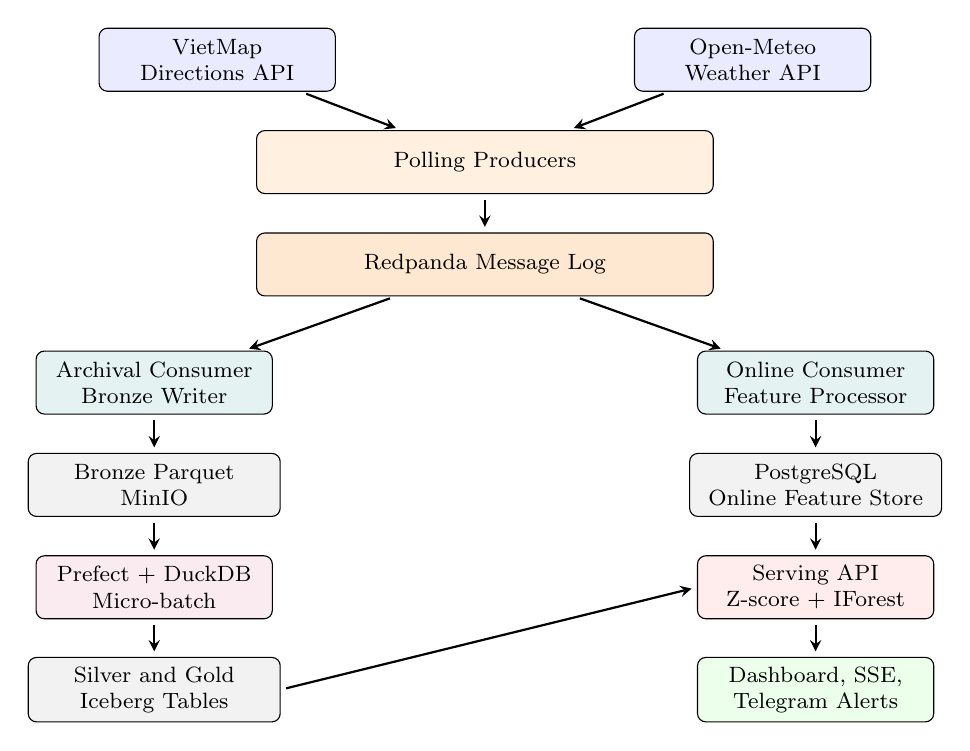
\begin{tikzpicture}[
        >=stealth,
        box/.style={draw, rounded corners=3pt, fill=white,
                    minimum width=3.0cm, minimum height=0.8cm,
                    align=center, font=\footnotesize},
        store/.style={draw, rounded corners=3pt, fill=gray!10,
                      minimum width=3.2cm, minimum height=0.8cm,
                      align=center, font=\footnotesize},
        arr/.style={->, thick, shorten >=2pt, shorten <=2pt}
      ]
        \node[box, fill=blue!8] (vietmap) at (-3.4,2.4) {VietMap\\Directions API};
        \node[box, fill=blue!8] (weather) at (3.4,2.4) {Open-Meteo\\Weather API};
        \node[box, fill=orange!12, minimum width=5.8cm] (producer) at (0,1.1)
          {Polling Producers};
        \node[box, fill=orange!18, minimum width=5.8cm] (redpanda) at (0,-0.2)
          {Redpanda Message Log};

        \node[box, fill=teal!10] (archival) at (-4.2,-1.7)
          {Archival Consumer\\Bronze Writer};
        \node[box, fill=teal!10] (online) at (4.2,-1.7)
          {Online Consumer\\Feature Processor};

        \node[store] (bronze) at (-4.2,-3.0) {Bronze Parquet\\MinIO};
        \node[box, fill=purple!8] (microbatch) at (-4.2,-4.3)
          {Prefect + DuckDB\\Micro-batch};
        \node[store] (silvergold) at (-4.2,-5.6)
          {Silver and Gold\\Iceberg Tables};

        \node[store] (postgres) at (4.2,-3.0)
          {PostgreSQL\\Online Feature Store};
        \node[box, fill=red!7] (serving) at (4.2,-4.3)
          {Serving API\\Z-score + IForest};
        \node[box, fill=green!8] (dashboard) at (4.2,-5.6)
          {Dashboard, SSE,\\Telegram Alerts};

        \draw[arr] (vietmap) -- (producer);
        \draw[arr] (weather) -- (producer);
        \draw[arr] (producer) -- (redpanda);
        \draw[arr] (redpanda) -- (archival);
        \draw[arr] (redpanda) -- (online);
        \draw[arr] (archival) -- (bronze);
        \draw[arr] (bronze) -- (microbatch);
        \draw[arr] (microbatch) -- (silvergold);
        \draw[arr] (online) -- (postgres);
        \draw[arr] (postgres) -- (serving);
        \draw[arr] (silvergold.east) -- (serving.west);
        \draw[arr] (serving) -- (dashboard);
      \end{tikzpicture}%
      }
      \caption{Dual-consumer data flow from Redpanda to Lakehouse and
      Online Feature Store.}                                                                                                                              
      \label{fig:data_flow}
  \end{figure}                                                                                                                                            
                  
  % ------------------------------------------------------------                                                                                          
  \subsection{Bronze Layer — Durable Event Archival}
  \label{subsec:bronze}
  % ------------------------------------------------------------                                                                                          
   
  The \texttt{apps/streaming} consumer buffers incoming Kafka messages in                                                                                 
  memory and flushes to \textbf{MinIO} object storage as \textbf{Apache
  Parquet} \cite{parquet_format} files using a \textit{dual-trigger flush                                                                                 
  policy}: a flush is issued when the buffer reaches 500 messages                                                                                         
  \textbf{or} when 30 seconds have elapsed since the last flush, whichever                                                                                
  occurs first. This policy bounds the maximum number of small files                                                                                      
  written — which degrades downstream query performance \cite{small_file_problem}                                                                         
  — and the maximum duration for which data remains unarchived in memory.                                                                                 
                                                                                                                                                          
  Kafka offsets are committed only after a confirmed successful MinIO                                                                                     
  upload (\texttt{asynchronous\allowbreak=False}). If an upload fails, the consumer                                                                                  
  does not advance its offset; messages are replayed on restart, providing                                                                                
  \textbf{at-least-once delivery} at the application level. Messages                                                                                      
  that cannot be processed after repeated attempts are routed to a                                                                                        
  \textit{dead-letter queue} (DLQ) topic (\texttt{\{topic\}-dlq}) for                                                                                     
  independent inspection and recovery \cite{enterprise_integration_patterns}.                                                                             
                                                                                                                                                          
  Parquet files are written with \textit{Snappy} compression and use                                                                                      
  a \textbf{Hive-style event-time partition scheme}:                                                                                                      
  \begin{center}                                                                                                                                          
  \texttt{bronze/traffic-route-bronze/year=Y/month=M/day=D/hour=H/\{uuid\}.parquet}
  \end{center}                                                                                                                                            
                  
  The partition key is derived from \texttt{timestamp\_utc} embedded in                                                                                   
  the observation itself — \textbf{not} the time of writing. This
  \textit{event-time partitioning} \cite{flink_event_time} ensures that                                                                                   
  late-arriving records are placed in the historically correct partition,                                                                                 
  preserving temporal integrity for all downstream aggregations.                                                                                          
                                                                                                                                                          
  % ------------------------------------------------------------
  \subsection{Silver Layer — Incremental Micro-Batch Processing}                                                                                          
  \label{subsec:silver}                                                                                                                                   
  % ------------------------------------------------------------
                                                                                                                                                          
  Every 5 minutes, the \texttt{microbatch} \textbf{Prefect}                                                                                               
  \cite{prefect_docs} flow executes a \textbf{DuckDB} \cite{duckdb_paper}
  scan over newly arrived Bronze Parquet files and promotes them to the                                                                                   
  Silver \textbf{Apache Iceberg} \cite{iceberg_paper} table                                                                                               
  (\texttt{silver.traffic\_route}), catalogued via \textbf{Project Nessie}                                                                                
  \cite{nessie_docs}.                                                                                                                                     
                                                                                                                                                          
  It is necessary to distinguish this stage from \textit{stateful stream                                                                                  
  processing} as implemented by systems such as Apache Flink                                                                                              
  \cite{flink_paper} or Spark Structured Streaming \cite{spark_streaming}.                                                                                
  The Silver layer uses an \textbf{incremental micro-batch} pattern: each
  Prefect run is a bounded, stateless DuckDB job that reads only files                                                                                    
  written since the last high-watermark and appends to Iceberg atomically.                                                                                
  This design was chosen deliberately: it eliminates the operational                                                                                      
  complexity of a long-running JVM streaming cluster while achieving Silver                                                                               
  freshness within 5 minutes of event arrival, which is sufficient given                                                                                  
  that the sub-second real-time path is served by the Online Feature Store                                                                                
  (Section~\ref{subsec:online}).                                                                                                                          
                                                                                                                                                          
  \textbf{Apache Iceberg} provides \textit{ACID-compliant snapshot isolation}:                                                                            
  concurrent readers observe a consistent table snapshot whilst a new                                                                                     
  micro-batch commit is in progress. It additionally supports                                                                                             
  \textit{schema evolution} (adding columns without invalidating existing                                                                                 
  readers) and \textit{time-travel} (querying the table at any previous                                                                                   
  snapshot by ID or timestamp) \cite{iceberg_paper}. These capabilities                                                                                   
  are foundational to the reproducibility requirement (NFR-2).                                                                                            
                                                                                                                                                          
  % ------------------------------------------------------------
  \subsection{Gold Layer — Hourly Aggregation}                                                                                                            
  \label{subsec:gold}                                                                                                                                     
  % ------------------------------------------------------------
                                                                                                                                                          
  Every hour, the \texttt{hourly-gold} Prefect flow aggregates the Silver                                                                                 
  table into \texttt{gold.traffic\_hourly}\allowbreak{} --- a pre-computed,
  per-hour summary. The Gold schema includes: \texttt{avg\_heavy\_ratio},                                                                                 
  \texttt{avg\_moderate\_ratio}, \texttt{avg\_duration\_minutes}, and                                                                                     
  \texttt{max\_severe\_segments}. DuckDB reads the Silver Iceberg table                                                                                   
  via the \textbf{PyIceberg} \cite{pyiceberg_docs} Arrow interface and                                                                                    
  writes results back to an Iceberg Gold table. The Gold layer serves                                                                                     
  two consumers: the \textit{IsolationForest training pipeline}                                                                                           
  (Section~\ref{subsec:iforest}) and the \textit{RAG traffic pattern                                                                                      
  indexer} (Section~\ref{subsec:rag_indexing}).                                                                                                           
                                                                                                                                                          
  % ------------------------------------------------------------                                                                                          
  \subsection{Online Feature Store — Real-Time Postgres Path}                                                                                             
  \label{subsec:online}
  % ------------------------------------------------------------                                                                                          
   
  In parallel with the archival path, the \texttt{apps/online} consumer                                                                                   
  maintains a live \textbf{Online Feature Store} in PostgreSQL
  (\texttt{online\_route\_features} table). For each Kafka message,                                                                                       
  the \texttt{OnlineFeatureProcessor} updates an in-memory hourly window                                                                                  
  for the corresponding route using \textbf{Welford's online algorithm}                                                                                   
  \cite{welford1962} — a numerically stable, single-pass method for                                                                                       
  computing a running mean and standard deviation without retaining the                                                                                   
  full observation history.                                                                                                                               
                                                                                                                                                          
  The Welford accumulator state is persisted to PostgreSQL on every                                                                                       
  message via an \texttt{UPSERT} keyed on \texttt{(route\_id, window\_start)}.
  On service restart, the processor reconstructs the accumulators from                                                                                    
  stored \texttt{mean}, \texttt{stddev}, and \texttt{count} via the
  inverse identity $M_2 = \sigma^2 \times (n-1)$, allowing accumulation                                                                                   
  to resume from the exact point of interruption rather than resetting                                                                                    
  the hourly window. Algorithm~\ref{alg:welford} formalises this procedure.                                                                               
                                                                                                                                                          
  \begin{algorithm}[H]                                                                                                                                    
      \small                                                                                                                                              
      \caption{$(\hat{\mu}, \hat{\sigma}, n) \gets                                                                                                        
      \texttt{WelfordUpdate}(x, \hat{\mu}_{\text{prev}}, M_{2,\text{prev}}, n_{\text{prev}})$}                                                            
      \label{alg:welford}                                                                                                                                 
      \begin{algorithmic}[1]                                                                                                                              
          \Require $x$ is the new heavy\_ratio observation for route $r$.                                                                                 
          \Require $\hat{\mu}_{\text{prev}}, M_{2,\text{prev}}, n_{\text{prev}}$                                                                          
          are the prior mean, sum of squared deviations, and count.                                                                                       
          \State $n \gets n_{\text{prev}} + 1$                                                                                                            
          \State $\delta \gets x - \hat{\mu}_{\text{prev}}$                                                                                               
          \State $\hat{\mu} \gets \hat{\mu}_{\text{prev}} + \delta \,/\, n$                                                                               
          \State $\delta_2 \gets x - \hat{\mu}$                                                                                                           
          \State $M_2 \gets M_{2,\text{prev}} + \delta \times \delta_2$                                                                                   
          \If{$n > 1$}                                                                                                                                    
              \State $\hat{\sigma} \gets \sqrt{M_2 \,/\, (n - 1)}$                                                                                        
          \Else                                                                                                                                           
              \State $\hat{\sigma} \gets 0$                                                                                                               
          \EndIf                                                                                                                                          
          \State \Return $(\hat{\mu},\; \hat{\sigma},\; n)$
      \end{algorithmic}                                                                                                                                   
  \end{algorithm}
                                                                                                                                                          
  \textbf{Crash recovery.} At startup, the processor queries PostgreSQL                                                                                   
  for the current hour's stored \texttt{mean}, \texttt{stddev},
  and \texttt{observation\_count} for each route and reconstructs                                                                                         
  the Welford state as:
                                                                                                                                                          
  \begin{equation}
  \label{eq:welford_recovery}                                                                                                                             
  M_2^{\text{recovered}} = \hat{\sigma}^2 \times \max(n - 1,\; 0)
  \end{equation}                                                                                                                                          
   
  This ensures that a mid-hour service restart does not discard partially                                                                                 
  accumulated statistics, satisfying fault-tolerance requirement NFR-3.
                                                                                                                                                          
  % ============================================================
  \section{Dual-Signal Anomaly Detection Framework}                                                                                                       
  \label{sec:anomaly}                                                                                                                                     
  % ============================================================
                                                                                                                                                          
  UrbanPulse employs two anomaly detection algorithms that are
  \textbf{mathematically orthogonal by design}: a \textit{univariate
  threshold-based} detector operating on the real-time feature stream,
  and a \textit{multivariate ensemble} detector trained on the historical
  Gold layer. Neither algorithm is a fallback for the other; they are
  fused at the serving layer to produce a three-tier confidence hierarchy.
  The rationale for combining both approaches follows from the observation
  that univariate methods miss complex joint anomalies, whilst ensemble
  methods lack the immediacy of per-message classification
  \cite{chandola2009anomaly}.

  Specifically, the two detectors address \textbf{complementary failure
  modes} of urban traffic anomaly detection:

  \begin{itemize}
    \item \textbf{Z-Score (univariate):} Monitors a single variable ---
    \texttt{heavy\_ratio}, the fraction of heavily congested road segments
    --- against a per-route, per-time-slot historical baseline. It detects
    \textit{acute statistical spikes}: situations where the current
    window's congestion intensity deviates sharply from what is normal at
    that hour on that route. Because it operates on a single dimension, it
    reacts within one Kafka message and is therefore suitable for
    \textit{immediate} alerting. Its weakness is blindness to
    \textit{multivariate} patterns: a route may appear normal on
    \texttt{heavy\_ratio} alone whilst simultaneously exhibiting
    abnormally elevated \texttt{moderate\_ratio} and
    \texttt{severe\_segments} --- a joint pattern invisible to univariate
    methods.

    \item \textbf{Isolation Forest (multivariate):} Operates on a
    7-dimensional feature space ($h_{\text{avg}}, m_{\text{avg}},
    s_{\text{max}}, h_{\sin}, h_{\cos}, d_{\sin}, d_{\cos}$) trained on
    the historical Gold layer. It detects \textit{distributional outliers}
    --- combinations of variables that are collectively rare given the
    route's historical traffic rhythm. It captures anomalies that unfold
    gradually (e.g., a sustained moderate congestion surge on a normally
    free-flowing suburban route during an atypical weekday), which a
    univariate Z-score threshold may not exceed. Its weakness is latency:
    scores are computed in batch every 15 seconds from a model retrained
    every 6 hours, rather than per-message.
  \end{itemize}

  The conjunction rule (\texttt{both\_anomaly} = Z-score $\wedge$
  IForest) is therefore a deliberate precision-recall trade-off: it
  sacrifices recall on events detectable by only one signal in exchange
  for a high-confidence, low-false-positive alert channel suitable for
  automated Telegram notification.                                                                                                                             
                                                                                                                                                          
  % ------------------------------------------------------------                                                                                          
  \subsection{Signal 1 — Z-Score Online Detector}
  \label{subsec:zscore}                                                                                                                                   
  % ------------------------------------------------------------                                                                                          
                                                                                                                                                          
  \paragraph{Rationale and Role.}
  Real-time anomaly detection requires a low-latency signal that responds instantly to traffic deviations. Z-score based on a rolling Welford baseline is ideal: it runs in $O(1)$ memory per route and produces per-message scores, capturing immediate spikes before batch models can react \cite{welford1962note, finch2009incremental}.

  \paragraph{Input, Configuration, Output.}
  The Online Service tracks a running mean of \texttt{heavy\_ratio} for each route using Welford's online algorithm, maintaining state $(n, \mu, M_2)$ in PostgreSQL. The batch baseline layer computes the 99th percentile of historical Z-scores ($p_{99,r}$) during the \texttt{baseline\_learning} job. For each incoming observation, the Z-score is:

  \begin{equation}
  \label{eq:zscore}
  z_r^{(t)} = \frac{\bar{h}_r^{(t)} - \mu_r^{\text{base}}}{\sigma_r^{\text{base}}}
  \end{equation}

  where $\bar{h}_r^{(t)}$ is the current Welford mean, and $\mu_r^{\text{base}}, \sigma_r^{\text{base}}$ are the batch baseline statistics. The adaptive threshold is:

  \begin{equation}
  \label{eq:threshold_rule}
  \theta_r = \max(1.5, \min(p_{99,r}, 2.0))
  \end{equation}

  The floor of 1.5 prevents excessive sensitivity on low-variance routes; the ceiling of 2.0 covers new routes lacking history. Classification is one-sided: only $z_r^{(t)} > \theta_r$ signals an anomaly (positive deviations indicate congestion; negative indicates free flow, which is not anomalous). The Z-score is stored in PostgreSQL's \texttt{online\_route\_features} table as \texttt{duration\_zscore} (schema legacy name retained for continuity) and exposed via the Serving Layer's WebSocket API.

  \begin{figure}[htbp]
      \centering
      
\includegraphics[width=\textwidth]{grafana-zscore-timeseries}
      \caption{Per-route Z-score over a 24-hour observation window
      (Grafana). Each line represents one directed inter-zone route.
      Spikes above the dashed threshold $\theta_r$ trigger the Z-score
      anomaly signal.}
      \label{fig:zscore_timeseries}
  \end{figure}

  % ------------------------------------------------------------
  \subsection{Signal 2 — Isolation Forest Batch Detector}                                                                                                 
  \label{subsec:iforest}
  % ------------------------------------------------------------

  \paragraph{Rationale and Role.}
  The dual-signal framework requires a second, independent detector to reconcile high-recall Z-score signals with high-precision multivariate outlier detection. Isolation Forest \cite{liu2008isolation} is well-suited for this role: it operates on a 7-dimensional feature space (congestion ratios + cyclical time encodings) without requiring labelled data or strong distributional assumptions, and its linear complexity in sample count enables 6-hourly retraining on homelab hardware \cite{isolation_survey_2025}.

  \paragraph{Input, Configuration, Output.}
  The feature vector per route-hour observation comprises three traffic metrics (avg heavy ratio, avg moderate ratio, max severe segments) and four cyclical time encodings (sine-cosine pairs for hour-of-day and day-of-week to ensure temporal circularity). An Isolation Forest model is trained every 6 hours on the Gold-layer corpus ($N \approx 1{,}600$ records per route) using Optuna Bayesian search to maximize the anomaly score gap.
                                                                                                                                                          
  \begin{equation}
  \label{eq:feature_vector}
  \mathbf{x} = (h_{\text{avg}}, m_{\text{avg}}, s_{\text{max}}, \sin(2\pi \cdot \text{hr}/24), \cos(2\pi \cdot \text{hr}/24), \sin(2\pi \cdot \text{dow}/7), \cos(2\pi \cdot \text{dow}/7))
  \end{equation}

  The cyclical encodings (sine-cosine pairs) ensure temporal circularity: hour 23 and hour 0 are geometrically adjacent, preventing false ordinal distances that would mislead the model about traffic periodicity.

  Table~\ref{tab:iforest_params} reports the resulting configuration.
  The \texttt{contamination} value of $0.01$ is consistent with an
  independent heavy-ratio Z-score anomaly rate estimate of $1.97\%$
  obtained by applying the statistical baseline rule to the same training
  corpus, providing cross-signal validation that
  genuine anomalous hours are rare in the pre-cutoff dataset.

  \begin{table}[htbp]
  \centering
  \caption{IsolationForest hyperparameters selected by Optuna TPE
           (50 trials $\times$ 20 routes; median aggregation).}
  \label{tab:iforest_params}
  \begin{tabular}{llll}
  \hline
  \textbf{Parameter} & \textbf{Search range} & \textbf{Default} & \textbf{Tuned} \\
  \hline
  \texttt{contamination} & $[0.01,\;0.15]$ & $0.05$ & $0.01$ \\
  \texttt{n\_estimators}  & $\{50,100,\ldots,500\}$ & $100$ & $450$ \\
  \texttt{max\_samples}   & $[0.5,\;1.0]$  & auto (${\approx}0.17$) & $0.76$ \\
  \texttt{max\_features}  & $[0.5,\;1.0]$  & $1.0$ & $0.73$ \\
  \hline
  \multicolumn{4}{l}{Mean score gap: default $0.059$ $\to$ tuned $0.083$
                     (+40.7\%, 20/20 routes improved).} \\
  \hline
  \end{tabular}
  \end{table}

  Figure~\ref{fig:optuna_validation} validates the tuned parameters against
  the default configuration across all 20 routes.
  The left panel plots tuned score gap against default score gap per route;
  all points lie above the diagonal, confirming improvement on every route.
  The right panel shows the distribution of score gap improvements
  (\texttt{tuned} $-$ \texttt{default}), with all values strictly positive
  (range $+0.01$ to $+0.047$, mean $+0.023$).

  \begin{figure}[htbp]
      \centering
      
\includegraphics[width=\textwidth]{optuna-validation}
      \caption{Optuna hyperparameter tuning validation across 20 routes.
      \textit{Left}: tuned vs.\ default anomaly score gap per route
      (all points above the diagonal indicate improvement).
      \textit{Right}: distribution of score gap delta
      (\texttt{tuned} $-$ \texttt{default}); all 20 routes show
      strictly positive improvement (mean $+0.023$, max $+0.047$).}
      \label{fig:optuna_validation}
  \end{figure}

  A lower \texttt{contamination} value raises the decision threshold,
  flagging only extreme outliers and biasing the detector towards
  precision; since dual-signal fusion (Section~\ref{subsec:fusion})
  handles recall via Z-score, IForest is tuned for
  high-confidence predictions. Every 6 hours, the model is retrained,
  registered in MLflow with the \texttt{@champion} alias, and loaded
  by the serving layer with a one-hour cache TTL.

  \begin{figure}[htbp]
      \centering
      
\includegraphics[width=\textwidth]{mlflow-experiments}
      \caption{MLflow experiment view showing per-route
      \texttt{IsolationForest} training runs for the
      \texttt{traffic-anomaly-detection} experiment.
      Each row corresponds to one directed inter-zone route model.}
      \label{fig:mlflow_experiments}
  \end{figure}


  % ------------------------------------------------------------
  \subsection{Dual-Signal Fusion}
  \label{subsec:fusion}                                                                                                                                   
  % ------------------------------------------------------------
                                                                                                                                                          
  The two signals are merged at the Serving Layer into a                                                                                                  
  \textbf{three-tier confidence hierarchy}. Let
  $z_r \in \{0, 1\}$ denote the Z-score anomaly label and                                                                                                 
  $f_r \in \{0, 1\}$ the IsolationForest anomaly label for                                                                                                
  route $r$. The fusion mapping is defined in                                                                                                             
  Algorithm~\ref{alg:fusion}.                                                                                                                             
                                                                                                                                                          
  \begin{algorithm}[H]
      \small                                                                                                                                              
      \caption{$\texttt{tier}_r \gets
      \texttt{SignalFusion}(z_r,\; f_r)$}
      \label{alg:fusion}                                                                                                                                  
      \begin{algorithmic}[1]
          \Require $z_r \in \{0, 1\}$ is the Z-score anomaly label.                                                                                       
          \Require $f_r \in \{0, 1\}$ is the IForest anomaly label.                                                                                       
          \If{$z_r = 1$ \textbf{and} $f_r = 1$}
              \State \Return \textbf{Tier 1}: \texttt{both\_anomaly}                                                                                      
              \Comment{Cross-validated; highest confidence}                                                                                               
          \ElsIf{$z_r = 1$ \textbf{and} $f_r = 0$}                                                                                                        
              \State \Return \textbf{Tier 2}: \texttt{zscore\_anomaly}                                                                                    
              \Comment{Immediate spike; may be transient}                                                                                                 
          \ElsIf{$z_r = 0$ \textbf{and} $f_r = 1$}
              \State \Return \textbf{Tier 3}: \texttt{iforest\_anomaly}                                                                                   
              \Comment{Multivariate pattern; not threshold-detectable}                                                                                    
          \Else
              \State \Return \textbf{Normal}                                                                                                              
          \EndIf                                                                                                                                          
      \end{algorithmic}
  \end{algorithm}                                                                                                                                         
                  
  Automated Telegram alerts are issued only for Tier 1 and Tier 3                                                                                         
  signals, filtered through a \textbf{30-minute per-route cooldown}
  managed in the \texttt{anomaly\_alert\_log} table. This threshold                                                                                       
  suppresses duplicate notifications during sustained congestion                                                                                          
  events whilst ensuring that any new independent anomaly episode                                                                                         
  triggers a fresh alert.                                                                                                                                 
                                                                                                                                                          
  % ============================================================                                                                                          
  \section{Knowledge-Enriched Inference via RAG}
  \label{sec:rag}                                                                                                                                         
  % ============================================================
                                                                                                                                                          
    The anomaly detectors in Section~\ref{sec:anomaly} output reliable
    numerical signals (Z-score and Isolation Forest labels), but those
    outputs alone are not sufficient for operational decision-making.
    Traffic operators need an explanation of \textit{why} congestion is
    occurring, not only whether an anomaly exists. UrbanPulse therefore
    applies \textbf{Retrieval-Augmented Generation (RAG)} \cite{lewis2020rag}
    as an interpretation layer that converts dual-signal alerts into
    root-cause narratives grounded in historical traffic behaviour and
    current weather context.

    % ------------------------------------------------------------
    \subsection{Role in the System (Why)}
    \label{subsec:vector_store}
    % ------------------------------------------------------------

    The role of RAG in UrbanPulse is strictly application-facing:
    \textbf{transforming raw anomaly alerts into actionable knowledge}.
    When an event is flagged, the system should answer a practical
    question for city operators: \textit{why is this route congested now?}
    In many cases, the explanation is compositional (for example, an
    unusual congestion spike coinciding with adverse weather during a
    peak-hour corridor). RAG is used to synthesise this multi-source
    context into concise natural language that can be consumed directly in
    dashboard workflows.

    % ------------------------------------------------------------
    \subsection{Implementation Pipeline (Input -- Configuration -- Output)}
    \label{subsec:rag_indexing}
    % ------------------------------------------------------------

    UrbanPulse implements RAG as a black-box inference pipeline with three
    operational stages:

    \begin{enumerate}
      \item \textbf{Input (Retrieval):} RAG is triggered for
      high-confidence events where both detection signals agree
      (\texttt{both\_anomaly}). The serving layer retrieves traffic
      context from ChromaDB (recent anomaly events and historical route
      patterns) and, in parallel, fetches current meteorological context
      from Open-Meteo.

      \item \textbf{Configuration (Model and Prompting):} Generation is
      executed by a local \textbf{Qwen2.5:3b} model served via
      \textbf{Ollama} \cite{qwen25_report,ollama_docs}. The local-LLM
      deployment is a deliberate infrastructure decision motivated by
      three constraints: municipal data privacy, predictable operating
      cost (no per-token external billing), and offline-capable
      deployment on city-controlled infrastructure. Retrieved traffic
      evidence and live weather variables are injected into a fixed prompt
      template together with numerical anomaly indicators
      (e.g., Z-score magnitude, congestion ratios, and route metadata).

      \item \textbf{Output (Generation):} The LLM returns a concise
      root-cause explanation in natural language, streamed via
      \textbf{Server-Sent Events} (SSE) \cite{sse_spec} and rendered
      directly in the operator interface (Grafana/UI) alongside the alert.
    \end{enumerate}

    This implementation is intentionally concise: from anomaly trigger to
    human-readable explanation in a single retrieval-augmentation-generation
    flow, without additional iterative reasoning loops in the serving path.
                                                                                                                                                          
  % ------------------------------------------------------------
  \subsection{Feedback Loop and Fine-Tuning Data Collection}                                                                                              
  \label{subsec:feedback}
  % ------------------------------------------------------------

  Every LLM interaction — query string, retrieved chunks with                                                                                             
  similarity scores, and the full generated response — is persisted
  to the \texttt{rag\_interaction\_log} PostgreSQL table. The                                                                                             
  \texttt{/rca/feedback} endpoint accepts a thumbs-up ($+1$) or                                                                                           
  thumbs-down ($-1$) rating per interaction, stored in the                                                                                                
  \texttt{feedback} column. This produces a continuously growing,                                                                                         
  human-labelled dataset suitable for future \textit{supervised                                                                                           
  fine-tuning} of the retrieval ranking or generation components                                                                                          
  \cite{rlhf_paper}, distinguishing UrbanPulse from systems that                                                                                          
  treat the LLM as a stateless inference endpoint.                                                                                                        
                                                                                                                                                          
  % ============================================================                                                                                          
  \section{Evaluation Framework}                                                                                                                          
  \label{sec:evaluation}                                                                                                                                  
  % ============================================================
                                                                                                                                                          
  The methodologies described in the preceding sections are designed                                                                                      
  to satisfy the three operational pillars established in
  Section~\ref{sec:requirements}: \textit{temporal integrity},                                                                                            
  \textit{reproducibility}, and \textit{observability}. This section                                                                                      
  defines the specific metrics and measurement boundaries that                                                                                            
  Chapter~4 will report.                                                                                                                                  

  \paragraph{Experimental Protocol.}
  The empirical evaluation follows a fixed protocol to ensure repeatable and comparable results. Traffic telemetry is collected continuously over a bounded observation window and retained at Bronze, Silver, Gold, and online-feature granularity. All experiments are executed on a single, fixed deployment environment; the hardware profile (CPU, memory, GPU, storage) and software stack (Docker, Python, Redpanda, PostgreSQL, MinIO, Iceberg/Nessie, MLflow, ChromaDB, Ollama) are recorded before each evaluation run.

  The workload profile consists of three measurement modes: (i) normal-load run using production polling and all routes, (ii) stress run replaying messages at $2\times$ throughput to assess stability, and (iii) inference run issuing repeated requests to measure latency under steady-state conditions. Baseline comparison is performed against a batch-only variant where anomaly labels become available only after periodic aggregation. For each metric, measurements are computed from persisted logs or monitoring systems using $p_{50}$, $p_{95}$, and max statistics.

  % ============================================================
  \subsection{Temporal Integrity}
  \label{subsec:eval_temporal}
  % ============================================================

  All Bronze Parquet files are partitioned by event timestamp.                                                                                            
  End-to-end ingestion lag $L_{\text{e2e}}$ is defined as:
                                                                                                                                                          
  \begin{equation}
  \label{eq:lag}                                                                                                                                          
  L_{\text{e2e}}^{(r,t)} = t_{\text{feature}} - t_{\text{ingest\_ts}}
  \end{equation}                                                                                                                                          
   
  where $t_{\text{ingest\_ts}}$ is the Unix millisecond timestamp                                                                                         
  recorded immediately before the VietMap API call (embedded in the
  Kafka message header) and $t_{\text{feature}}$ is the time at which                                                                                     
  the corresponding \texttt{UPSERT} completes in PostgreSQL. This metric
  is exposed per-route and aggregated at \texttt{/online/lag} as                                                                                          
  $p_{50}$, $p_{95}$, and $\max$. The target for NFR-1 is                                                                                                 
  $L_{\text{e2e}}^{p_{95}} < 20\,\text{s}$.                                                                                                               
                                                                                                                                                          
  % ------------------------------------------------------------                                                                                          
  \subsection{Reproducibility}                                                                                                                            
  \label{subsec:eval_reproducibility}
  % ------------------------------------------------------------

  Two mechanisms jointly ensure reproducibility. First, the                                                                                               
  \textbf{Apache Iceberg} time-travel API allows any Silver or
  Gold table to be queried at any historical snapshot by ID                                                                                               
  or timestamp — meaning the exact data state at the time of
  any anomaly classification can be reconstructed. Second,                                                                                                
  \textbf{MLflow} records the full provenance of every
  IsolationForest training run: hyperparameters
  (\texttt{contamination}, \texttt{n\_estimators},
  \texttt{max\_samples}, \texttt{max\_features},
  \texttt{random\_state}, \texttt{training\_cutoff}),
  feature schema, and training data time
  range; therefore, each inference can be replayed against the same
  model version and data snapshot.                                                                                                                                          
                                                                                                                                                          
  % ------------------------------------------------------------                                                                                          
\subsection{Performance Metrics}
  \label{subsec:performance_metrics}
  % ------------------------------------------------------------
                
  The following metrics summarise the system's ability to satisfy the operational pillars:
            
  \begin{table}[h]
  \centering
  \caption{Performance metrics: temporal integrity, reproducibility, and system performance}
  \label{tab:performance_metrics}
  \resizebox{\textwidth}{!}{%
  \begin{tabular}{llll}
  \hline               
  \textbf{KPI} & \textbf{Definition} & \textbf{Target} &                                                                                                  
  \textbf{Measurement point} \\                         
  \hline                                                                                                                                                  
  Ingestion lag $p_{95}$    & $t_{\text{feature}} - t_{\text{ingest\_ts}}$
                            & $< 20\,\text{s}$                                                                                                            
                            & \texttt{/online/lag} \\                                                                                                     
  Microbatch freshness      & Bronze write $\to$ Silver commit
                            & $< 5\,\text{min}$                                                                                                           
                            & Prefect task duration \\                                                                                                    
  IForest scoring latency   & Background scorer cycle
                              duration (15\,s interval)
                            & $< 5\,\text{s}$
                            & Serving API logs \\                                                                                                         
  \hline                                                                                                                                                  
  \end{tabular}
  }%
  \end{table}                                                                                                                                             
                                                                                                                                                          
  By integrating periodic high-velocity API polling with an incrementally
  processed, versioned Data Lakehouse and two independent, orthogonal                                                                                     
  anomaly detectors, the methodology presented in this chapter provides
  a rigorous foundation for evaluating UrbanPulse's ability to maintain                                                                                   
  low-latency, reproducible situational awareness under real-world                                                                                        
  metropolitan workloads in Ho Chi Minh City.                                                                                                             
                                                                                                                                                          
 
